\documentclass[a4paper,12pt]{scrartcl}
\usepackage[utf8]{inputenc}
\usepackage[T1]{fontenc}
\usepackage{lmodern}
\usepackage{amsmath}
\usepackage{amssymb}
\usepackage{makeidx}
\makeindex{}
\usepackage{hyperref}
\usepackage{csquotes}
\usepackage{graphicx}

\usepackage[backend=biber,style=numeric]{biblatex}
\addbibresource{bibliography.bib}


%\renewcommand{\thesection}{Sitzung \Roman{section}: }
%\usepackage{titlesec}
%\titlelabel{Sitzung \thesection{} --- }
\title{Human Factors in Security and Privacy}
\author{\href{mailto:magnus.berendes@fau.de}{magnus.berendes@fau.de}}
\date{\today}
\begin{document}
\maketitle

\vfill
\begin{centering}
	Corrections, annotations and pull requests appreciated
	\\
\end{centering}


\newpage

\tableofcontents
\newpage
\printindex
\printbibliography
\newpage

\section{Introduction}
\begin{itemize}
	\item
		What is security?\index{Security}
		\begin{itemize}
			\item
				Protect the right thing in a right way (Anderson)
			\item
				Risk management: Trade-off between risk of attack and cost of protection
		\end{itemize}
	\item
		Defining Security:
		\begin{itemize}
			\item
				Goals: \textit{what} to protect

				Security properties of assets: CIA\index{CIA} (Confidentiality, Integrity, Availability)
			\item
				Threats: \textit{against what/whom} to protect
			\item
				Means: \textit{how} to protect

				Safeguards (attack prevention) and Countermeasures (detection and response)
		\end{itemize}
	\item
		Human Factors as Protection Means:
		\begin{itemize}
			\item
				Security management processes: policies, rules, decisions
			\item
				Usable security
			\item
				User education and training (apply with care!)
		\end{itemize}

	\item
		Security-questions to ask:
		\begin{itemize}
			\item
				System:
				\begin{itemize}
					\item
						Technical structure/organization
					\item
						Stakeholders: user types, service providers
					\item
						Assets: what should be protected?
				\end{itemize}
			\item
				Security goals? CIA?
			\item
				Threats/Attackers?
				\begin{itemize}
					\item
						Which threats are possible, probable, incur high losses?
					\item
						Incentives of the attackers?
					\item
						Resources/capabilities of the attackers?
				\end{itemize}
			\item
				Does the security measure protect against these attacks?
			\item
				If yes, is the protection \textit{effective}?
				\begin{itemize}
					\item
						Cost of protection vs. attack risk
					\item
						Are users capable of the required behavior?
				\end{itemize}
			\item
				Is it \textit{efficient}?
				\begin{itemize}
					\item
						Cost of protection (money, time, user effort (!) ) vs. attack risk
				\end{itemize}
		\end{itemize}
	\item

		\begin{figure}[ht]
			\centering
			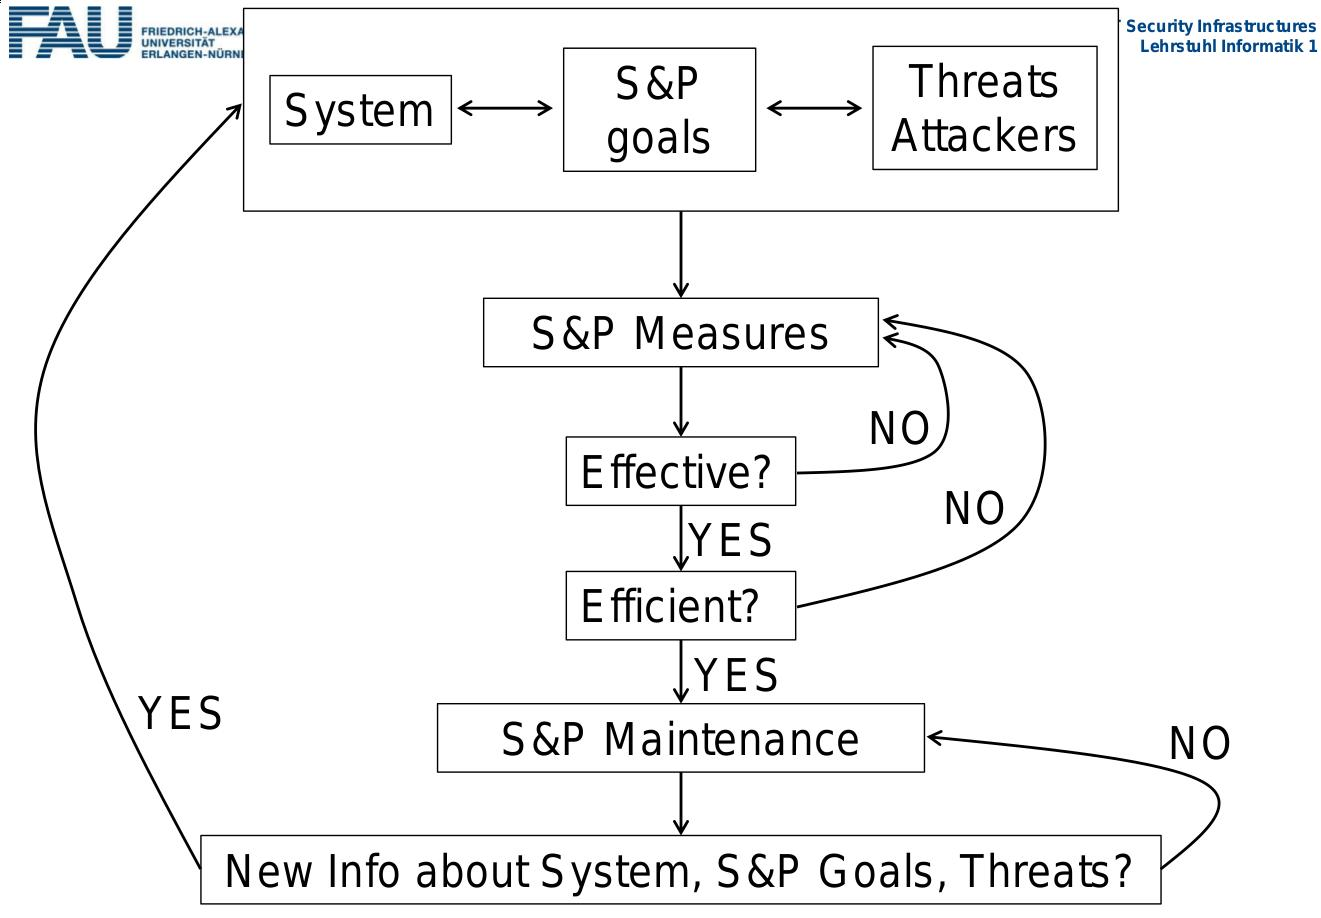
\includegraphics[
			width=0.8\textwidth]{security_process.jpg}
		\end{figure}

	\item
		Many S\&P measures offer bad trade-offs to the user: not much (subjective) gain of security, but a hassle
	\item
		\textit{Authorization}: \index{Authorization}
		\begin{itemize}
			\item
				Identification (e.g. login name)
			\item
				Plus authentication (e.g. password)
		\end{itemize}
\end{itemize}



\section{Passwords}
\begin{itemize}
	\item
		Security goals:
		\begin{itemize}
			\item
				Keep the bad guys out
			\item
				Don't lock me out!
		\end{itemize}
	\item
		Traditional password advice: strong (hard to guess), don't use it anywhere else, don't write it down, don't share it, change it often
	\item
		Do people follow this advice? No!
\end{itemize}
\subsection{Users are not the enemy}
\begin{itemize}
	\item
		\fullcite{usersenemy}
	\item
		Asked users about their password construction, frequency of use of different passwords, password recall
	\item
		Password diaries: write down all \enquote{happenings} around the password based authentication
	\item
		Findings:
		\begin{itemize}
			\item
				Users do not comply with policies
			\item
				but are not being wicked or stupid:
			\item
				They lack the right mental models of threats
			\item
				Password mechanisms lack user-centered design: not aligned with human memory capacities, not aligned with workflows (working together, delegating)
		\end{itemize}

		$\Rightarrow$ People chose weak passwords, reuse passwords, write them down, share them
	\item
		Mental Model \index{Mental Model}:
		\begin{itemize}
			\item
				Internal symbolic representation of external reality
			\item
				E.g. password=key model (how do i know if the website I'm logging into is real or fake? The key fits!)
			\item
				\enquote{Hackers cannot know the name of my cat, therefore that's a safe password}
		\end{itemize}
\end{itemize}

\subsection{A large-scale study of web password habits}
\begin{itemize}
	\item
		\fullcite{florenciolarge}
	\item
		544960 web clients, 3 months
	\item
		Windows Live Toolbar component with opt-in
	\item
		Report findings: websites, password compostion statistics (passwords were not transmitted), reuse, number of login attempts, time since last login
	\item
		Numnber of accounts per user: 25
	\item
		Each password shared across 4 different sites (avg)
	\item
		Passwords used per day: 8
	\item
		Mostly only lowercase letters \textit{unless forced to do otherwise}
\end{itemize}

\subsection{Passwords \& Human capabilities}
\begin{itemize}
	\item
		Why password logins fail:
		\begin{itemize}
			\item
				Failure to recall pssword

				Limited capacity of memory, decay over time, only unaided recall (no cues), items are non-meaningful, passwords are confused (items are similar and compete in memory), remember old password
			\item
				Typing errors

				no feedback on failure, needs to be 100\% correct
			\item
				Incorrect User ID
			\item
				User ID $\leftrightarrow$ password confusion
			\item
				Lock out after 3 attemps:

				Increasing to 10 tries decreases resets by 45\%
		\end{itemize}
	\item
		\fullcite{inglesanttrue}
		\begin{itemize}
			\item
				Data collection:  password diaries and interviews at two companies
			\item
				Conclusion very similar to \enquote{Users are not the enemy} from 1999 --- no positive changes after 10 years
		\end{itemize}
	\item
		\fullcite{florenciosecurity}
		\begin{itemize}
			\item
				Policies concentrate on forcing users to produce \enquote{strong} passwords
			\item
				Analysed \index{Minimal strength of password policies} minimal strength of password policies over 75 websites
			\item
				Minimal strength of a password policy: $N_{min} \log_2 C$

				$N_{min}$: minimal length, $C$: Character Space
			\item
				Analyses strength of the policy, not the password (strength of \enquote{password} is roughly the same as of \enquote{p4\$\$w0rd}, policy of the latter is much stronger)
		\end{itemize}
	\item
		Strength of password policies in the wild: FAU IdM much stronger than the rest ($48 > 20-27$)

		Sites with advertising often much weaker policies $\Rightarrow$ want user to sign up, password policies prevent that!
\end{itemize}
\subsection{Attacks on passwords}
\begin{itemize}
	\item
		Client: local attacks (shoulder surfing, post-its), social engineering, keyloggers
	\item
		Network:
		eavesdropping, MitM
	\item
		Server frontend: Online guessing (brute-force/dictionary) --- breadth-first (target all accounts), depth-first (target particular account), stealthy attacks (distributed in time)
	\item
		Server backend: offline guessing (prerequisite: obtain password database)
	\item[$\Rightarrow$] strong password policies protect against offline guessing attacks --- offline guessing attacks only feasible when password database is leaked, leak is not detected and passwords are salted and hashed
	\item
		Lookup tables/Rainbow tables: TODO
		\begin{itemize}
			\item
				Pre-compute hashes of passwords and look them up
			\item
				Password spaces quite big (10 ULNS policy needs more than $2^{65}$ hashes $ \mathrel{\widehat{=}} 1000$ Exabyte)
		\end{itemize}
	\item
		Online-offline chasm:
		\begin{itemize}
			\item
				Strength of passwords against online guessing: $10^4 - 10^6$ guesses
			\item
				Strength of passwords against offline guessing: $10^{14} - 10^{20}$ guesses
		\end{itemize}
		
	\item
		Summary to strong passwords:

		Strong passwords\dots
		\begin{itemize}
			\item
				reduce risk of offline guessing (iff database is hashed and salted)
			\item
				reduce risk of online guessing (but with lock-out and monitoring much weaker passwords are sufficient)
			\item
				might reduce risk against shoulder surfing and insider guessing
			\item
				don't protect against: malware, phishing, network attacks
			\item
				might increase risk of password reuse and writing down
		\end{itemize}
\end{itemize}

\subsection{Password Reuse}
\begin{itemize}
	\item
		\fullcite{tangledpasswordreuse}
		\begin{itemize}
			\item
				Study of password reuse with leaked passwords from eleven web sites
			\item
				Lots of reuses: 43\% identical, 19\% substrings
			\item
				Often tricks to transform passwords to comply with policies
		\end{itemize}
	\item
		\fullcite{florencio2014password}
		\begin{itemize}
			\item
				Lots of effort to remember which password belongs to which account \\
				($\log_2(N!)$, for N unique and random passwords)
			\item
				Unique passwords is not the optimal solution $\Rightarrow$ optimally, people should reuse passwords, group by account value and probability of compromise
		\end{itemize}
	\item
		Password Sharing
		\begin{itemize}
			\item
				Reasons for password sharing: practical needs (if something happens to me, delegation, disabilities), social norms (as a sign of trust, to show you're not paranoid, I'm a normal, nice, helpful person)
		\end{itemize}
	\item
		Password Change
		\begin{itemize}
			\item
				\fullcite{zhang2010security}
			\item
				Access to expired passwords at university, assuming knowledge of at least one password, guessed 17\% in 5 tries or lower (online), 41\% in under 3 seconds of offline attacking
		\end{itemize}
	\item
		Password Management 101
		\begin{itemize}
			\item
				Providers:
				\begin{itemize}
					\item
						Reasonable password policies and SSO
					\item
						Protection from offline guessing (hashed and salted, detect offline attacks e.g. with decoy accounts)
					\item
						Protection from online guessing (lock out after some failures, detect stealth attacks)
					\item
						Be prepared (usable and secure account recovery mechanisms, actionable strategies for the case of mass breaches)
				\end{itemize}
			\item
				Users
				\begin{itemize}
					\item
						Group passwords by account importance and attack probability (non important passwords can be reused; are users capable of distinguishing non/important accounts? Of determining attack probability?)
					\item  
						Don't reuse passwords on really important accounts
					\item
						Use aids for password management (password managers, secure writing down)
				\end{itemize}
		\end{itemize}
	\item
		Alternatives to passwords: graphical authentication, biometrics, tokens, 2FA
\end{itemize}

\section{Usable Security}
\begin{itemize}
	\item
		Usability: the extent to which a product can be used by specified users to achieve specified goals with effectiveness, efficiency and satisfaction in a specified context of use.
		\begin{itemize}
			\item
				Effectifeness: accuracy and completeness
			\item
				Efficiency: resources expended in relation to accuracy and completeness
			\item
				Satisafction: freedom from discomfort, and positive attitude to use of product
			\item
				context of use: characteristics of the users, tasks and environment
			\item
				Goal: intended outcome
			\item
				Task: activities required to achieve a goal
		\end{itemize}
	\item
		Usability Intervention at IBM 1989
		\begin{itemize}
			\item
				Field study: user group, environment, task (not authenticate, but \textit{do these 4 transactions})
			\item
				3 iterations (from mock-up to test code)
			\item
				100\% return on invested money, through time  saved while authenticating
		\end{itemize}
	\item
		\fullcite{johnnyencrypt}
		\begin{itemize}
			\item
				Security software is usable if people who are expected to use it:
				\begin{enumerate}
					\item
						Are reliably made aware of the security tasks they need to perform
					\item
						are able to figure out how to successfully perform those tasks
					\item
						don't make dangerous errors
					\item
						are sufficiently comfortable with the interface to continue using it
				\end{enumerate}
			\item
				experienced email users, no knowledge in cryptography in a lab, 12 participants
		\end{itemize}
	\item
		\fullcite{johnny2015}
		\begin{itemize}
			\item
				10 pairs of students, exchange tax return information with Mailvelope
			\item
				Results desastrous, only 1 pair completed the task (one of them knew about public key crypto before)
			\item
				All without attacker interference!
		\end{itemize}
	\item
		\fullcite{johnny2}
		\begin{itemize}
			\item
				Send sensitive data with Outlook and S/MIME, certificates are pre-loaded into mail clients of participants
			\item
				Participants don't know they are going to be attacked
			\item
				New Key attack: \enquote{computer problems}, send schedule to new address, new address has unmatching key from old address
			\item
				New Identity attack: \enquote{working from home}, new hotmail email with a new public key and misspelled email address (sara instead of sarah)
			\item
				Unsigned message attack: attacker impersonates manager being annoyed, known address, unsigned mail. Send schedule to team members NOW as they really need it
			\item
				3 groups: unmodified outlook, outlook with color coding (for secure and unsecure messages) and color coding + briefing about meaning of colors
			\item
				Conclusion: usable email clients help \textit{sometimes}: resisting attacks better with color/color+briefing, clicked encrypt is worse than with unmodified

				Some users did not trust \textit{hotmail}, ability to encrypt a message for the sender taken for indicator that the sender is genuine
		\end{itemize}
	\item
		Why is usable security hard?

		Usability: the extent to which a product can be used by specified users to achieve specified goals with effectiveness, efficiency and satisafaction in a specified context of use
		\begin{itemize}
			\item
				Product: Security is often integrated/part of product
			\item
				User Goals: Security = secondary goal
			\item
				Effectiveness: how can security be noticed? Often invisible
			\item
				Efficiency: additional time \& user effort
			\item
				Satisfaction: can people be satisfied with something that demands additional effort? Maybe better: low dissatisfaction?
			\item
				context of use: How to take attacks into account?
		\end{itemize}
	\item
		Benenson defintion of usable security:
		\begin{itemize}
			\item
				Usability of a security mechanism or policy
			\item
				is the extent to which the machnism or policy can be used by
			\item
				specified users
			\item
				to achieve the specified security goal (some of these goals being invisible or secondary goals to the users)
			\item
				and the specified primary goals
			\item
				with effectiveness, efficiency and satisfaction (or at least with low dissatisfaction)
			\item
				during the execution of the specified primary user tasks
			\item
				in a specified context of use
			\item
				including the specified attacks
		\end{itemize}
\end{itemize}
\subsection{Beyond Usability}
\begin{itemize}
	\item
		Is usability \& security a trade-off? long random passwords, single password per account, encrypted email, \dots
		\begin{itemize}
			\item
				Security versus Usability: security restricts/prohibits, usability enables
			\item
				Security aligned with Usability: Usability enables actions with desirable results, security restricts actions with undesirable results
		\end{itemize}
	\item
		Can't just add security to finished product $\Rightarrow$ usability will suffer
	\item
		Approaches to usable security (Apply in this order!)
		\begin{itemize}
			\item
				Invisible security: Make it just work, automated and invisible
			\item
				Understandable security: Make it visible and intuitive
			\item
				Train the users: effort should match benefit
		\end{itemize}
	\item
		Alternatives to passwords for web authentication:
		\begin{itemize}
			\item
				Criteria: Usability; Security/Privacy; Deployability
			\item
				Evaluated 35 alternative techniques: graphical passwords/PINs, Biometrics, Tokens, 2FA
			\item
				Results: many techniques would be better for security and privacy buuuut none has better deployability (for Web)
		\end{itemize}
	\item
		Usability criteria for web authentication:
		\begin{itemize}
			\item
				Memorywise (quasi) effortless
			\item
				Scalable for users (many accounts)
			\item
				Nothing to carry (or something the user carries anyway)
			\item
				Physically effortless (beyond pressing a button)
			\item
				Easy to learn
			\item
				Efficient to use (time)
			\item
				Infrequent errors
			\item
				Easy recovery from loss
		\end{itemize}

		Security and privacy criteria: resilience to
		\begin{enumerate}
			\item
				Physical observation
			\item
				targeted impersonation (having personal info about user does not help)
			\item
				throttled guessing (guessing attempts are constrained by service provider)
			\item
				Unthrottled guessing (attacker constrained only by computational resources)
			\item
				Internal observation (intercept users input)
			\item
				Leaks at other service providers
			\item
				Phishing
			\item
				theft of physical token (or at least pin protection)
			\item
				No trusted third party
			\item
				Explicit consent (authentication cannot be startet without user knowledge or consent)
			\item
				Unlinkable (colluding service providers cannot track the users from their authentication data)
			\item
				Privacy-protecting (does not reveal additional information about the user to the service provider / attacker
		\end{enumerate}

		Deployability Criteria
		\begin{enumerate}
			\item
				Accessible
			\item
				Low cost per user
			\item
				Server-compatible
			\item
				Browser-compatible
			\item
				Mature (User testing, open source implementations, real-world deployments)
			\item
				Non-proprietary
		\end{enumerate}
	\item
		Why doesn't Jane protect her Privacy? Renaud et.al.
		\begin{itemize}
			\item
				Qualitative study
		\end{itemize}
\end{itemize}

\section{Cyberfraud}
\begin{itemize}
	\item
		Fraud: crime of intentional deception
	\item
		Phishing: gain secret information (often via email)
	\item
		Scam: gain money (f2f/long distance: letters, emails)
	\item
		Social engineering: manipulate people. Gain information, make them perform action
\end{itemize}
\subsection{Phishing}
\begin{itemize}
	\item
		\fullcite{socialphishing}
		\begin{itemize}
			\item
				Crawl online social network sites, send phishing email with a link 
				and \enquote{hew, check this out!}
			\item
				Social phishing group: from an OSN friend, control group: \enquote{Normal} phishing
			\item
				Ask to log into website with phishy link, forward credentials to real website
			\item
				Results:
				\begin{itemize}
					\item
						Control group: 16\% phished, Social phishing group: 72\% phished
					\item
						Big ethics outcry: students were not aware they participated in the experiment, only prof, Insitutional Review Board and 2 IT guys knew
					\item
						Students who were phished complained (university took their trust and threw it out of the window) and students whose emails were used to phish, IT Department
				\end{itemize}
		\end{itemize}
	\item
		\fullcite{jakobsson2008}
		\begin{itemize}
			\item
				Harm done? Credentials obtained? Other forms?
			\item
				Informed consent before the experiment obtained?
			\item
				Debriefing: yes or no? What causes more harm?
		\end{itemize}
	\item
		\fullcite{downs2006decision}
		\begin{itemize}
			\item
				How do people decide over trustworthiness of emails?
			\item
				20 participants, role playing, didn't know experiment was about phishing or scam
			\item
				Results 
				\begin{enumerate}
					\item
						This email seems to be for me
					\item
						It's normal to hear from companies you do business with
					\item
						Reputable companies will send emails
				\end{enumerate}

		\end{itemize}
	\item
		\fullcite{2006phishing}
		\begin{itemize}
			\item
				20 e-commerce or banking websites (7 real, other collected or constructed)
			\item
				22 participants, distinguish which sites are fake
			\item
				Good phishing worked on 90\% of users
			\item
				Certificate warnings and security indicators were ignored a lot
			\item
				Independent of education, age, sex, computer experience
			\item
				Decision strategies: Security indicators in website content only, Content and domain name only, Content and address, plus \textsc{https}, All the above plus padlock icon, All the above plus certificates (kind of sorted by strength)
		\end{itemize}
	\item
		\fullcite{2015phishing}
		\begin{itemize}
			\item
				Lab experiment, identify phishing websites
			\item
				Participants average success rate of 53\% for identifying phishing websites $\Rightarrow$ guessing
			\item
				While making decisions, only 6\% of time looking at security indicators, 85\% looking at contents of webpage
			\item
				Technical proficency does not correlate with improved detection scores
		\end{itemize}
	\item
		Spear-Phishing: Trageting a group / an individual (by name, spoof trusted sender, plausible content)
	\item
		Studies by Benenson et.\ al.
		\begin{itemize}
			\item
				Questions:
				\begin{itemize}
					\item
						Email vs. Facebook, differences in attack effectiveness
					\item
						Reasons for clicking and not clicking?
				\end{itemize}
			\item
				Consent \& Deception: participants recruited for survey about \enquote{online behavior} + Debriefing about real aim of study
			\item
				Study 1 (with name): more effective via email
			\item
				Study 2 (without name): more effective via facebook
			\item
				Nach (nicht-)klicken Nachricht mit Bitte warum (nicht) geklickt wurde
			\item
				Analysemethode der Antworten: 
				\begin{itemize}
					\item
						Qualitative Content Analysis
					\item
						Iteratice Coding
					\item
						2 Raters and Cohens Kappa\footnote{How much the correlation between the 2 ratings differs from random}
				\end{itemize}
			\item
				Reasons for clicking:
				\begin{itemize}
					\item
						Curiosity / interest (34\%)
					\item
						Plausible content, fits expectations (27\%)
					\item
						Investigation (17\%)
					\item
						Technical context, Fear, Automatic reaction
				\end{itemize}
				
			\item
				What makes people click:
				\begin{itemize}
					\item
						Personalization
					\item
						Plausible content and context
					\item
						Emotions: curiosity, interest, fear
					\item
						Risk underestimation
					\item
						automatic reactions
				\end{itemize}
			\item
				reasons for not clicking:
				\begin{itemize}
					\item
						Unknown sender, suspicion of fraud, situation context, life context, rule of conduct, privacy
				\end{itemize}
		\end{itemize}
	\item
		Measures against Phishing
		\begin{itemize}
			\item
				Invisible Security
				\begin{itemize}
					\item
						Detection an blocking on provider side: takes up to 12 hours, lots of clicks in the first 2 hours, links  mostly work for less than 24 hours
					\item
						Automatic detection on user side: too many false negatives and false positives
				\end{itemize}
			\item
				Understandable security:
				\begin{itemize}
					\item
						Indicators / warnings
					\item
						Poor accuracy of automatic detection
					\item
						People do not notice, get habituated
				\end{itemize}
			\item
				Training / education: What is feasible / effective?
		\end{itemize}
	\item
		Awareness Requirements on Users: Be suspicious, even if you know the sender, the message fits your current situation and fits your work and life practices

		Be suspicious of everything!
	\item
		Decision making by Kahneman: two ways System 1 (intuition, effortless) and System 2 (rational reasoning)
	\item
		Can we make users aware by catching them on insecure behavior? Phishing as a service?
		\begin{itemize}
			\item
				2015 Police division in Berlin
			\item
				Email: Store all your work and private passwords in the secure password storage of the Berlin police. Corporate Design, Signature from non-existing person
			\item
				Half of subjects clicked, 7.5\% gave their credentials (35 individuals)
			\item
				Technical solution: visually distinguish internal \& external emails to help the users, save effort and avoid mistakes
		\end{itemize}
	\item
		Why is (Spear) phishing awareness difficult?
		\begin{itemize}
			\item
				Security aware behavior is difficult to maintain (constant vigilance, system 2) is tiring and unhealthy
			\item
				Life and work practices clash with expected security behavior: people receive lots of attachments, how can they distinguish legitimate ones? Lots of (wasted?) time, when checking every link received
			\item
				Social norms clash with expected security behavior (\enquote{what would they think if I [insert security behavior]}) See door policy
				
		\end{itemize}
	\item
		Countermeasures: What do you want people to \emph{do}? Will they be \emph{able} to do this? Effects on Producitvity, well-being, trust relationships. Evidence needed!
	\item
		Should we train users at all? Is the defense worth the effort?
	\item
		\fullcite{herley2009so}
		\begin{itemize}
			\item
				Fully rational individual user should reject most of the security advice existing today. Focus on individual users, not businesses
			\item
				Cost-benefict calculations:
				\begin{itemize}
					\item
						Protect from direct costs: attacks --- small or unknown costs
					\item
						Burden with indirect costs (externalities) through following security advice --- larce costs (time, nerves, money)
				\end{itemize}
			\item
				US phsihing annual costs of \$60 million
			\item
				US online population of 180 million users
			\item
				33 cents per person per year
			\item
				With minimum wage, anti-phishing education should be 2.6 minutes annually
		\end{itemize}
	\item
		And in Germany?
		\begin{itemize}
			\item
				Phishing Cost 2014 (peak): 27.9 million EUR
			\item
				Online Banking Users: 37 million people
			\item
				75 cents per year
			\item
				5.3 minutes per year
		\end{itemize}
	\item
		Pishing Risk = probability of attack * cost of attack
		\begin{itemize}
			\item
				Probability of being phished: 7000 cases in 2014, $37\times10^6$ customers $\Rightarrow$ 0.0002
			\item
				Expected cost of being phished: 28 Mio / 7000 cases = 4000 EUR per case
			\item
				Expected effort for getting money back if phished: 1 day (8 h), 1 week (40 h), 5 weeks (200h)?

				Average wage is 20 EUR/h, even with 5 weeks only 4000 Euro
			\item
				Risk of being phished = probability of attack * cost of attack $\Rightarrow 0.0002 \times4000 = 0.8$ EUR
			\item
				Only applicable for individual users, not businesses
		\end{itemize}
	\item
		RSA breach (2011)
		\begin{itemize}
			\item
				Started with spear phishing emails to small groups of employees (not high profile or high value target)
			\item
				One employee in HR received mail out of their junk folder (to make attack detection more difficult), double-clicked on the email attachement (because fits job expectation, curiosity)
			\item
				Consequences: SecureID maybe hacked, very popular 2FA tool, 40 millions tokens changed

				70 Million USD spent on aftermath of attack  
			\item
				Perimeter security (don't let attackers in!) failed, but in-depth defenses worked
		\end{itemize}
	\item
		Feasibility of Anti-Phishing Training
		\begin{itemize}
			\item
				Perimeter defense against spear phishing is difficult (exploit indispensable human characteristics, heuristics, work and life practices)
			\item
				False negatives: How to tell a fraud attempt from legitimate requests?
		\end{itemize}
	\item
		Effectiveness of Anti-Phishing Training: 50\%$\rightarrow$75--85\% with students.

		No evidence of effectiveness in real-world business environment
\end{itemize}
\subsection{Scam}
\begin{itemize}
	\item
		\fullcite{herley2012nigerian}
		\begin{itemize}
			\item
				Somebody who believes this, can be made to believe anything; somebody who does not fall for this is not worth the effort, at some point the are likely to notice that this is a scam
		\end{itemize}
	\item
		\fullcite{lea2009psychology}
		\begin{itemize}
			\item
				Study about scams in the UK, Interview with Scam Victims, Text Mining of scams, Scam Simulation
			\item
				Features of Scam Victims
				\begin{itemize}
					\item
						Better than average knowledge and experience in the scam (prize draws, lottery, investments) area 
					\item
						Lack of emotional control

					\item
						More effort in cognitive analysis of Scam (\enquote{Is this a good offer? Should I? Why? Why not?})
					\item
						Long-odds gamble: little to loose, a lot to win? (Misunderstanding: cannot win)
					\item
						Hiding response to scam, even from their more rational selves
				\end{itemize}
			\item
				How Scam works:
				\begin{itemize}
					\item
						Appeals to trust and authority
					\item
						Visceral triggers (personalization, big money, urgency --- provoke intuitive reactions, reduce thinking)
					\item
						Scarcity cues (urgency and uniqueness)
					\item
						Behavioral commitment (small steps of compliance --- sunken cost fallacy?)
					\item
						Disproportion between prize and cost/effort --- phantom fixation: concentrate on the huge prize
				\end{itemize}
			\item
				Conclusions:
				\begin{itemize}
					\item
						Scam victims have distinct psychological features, but not bad decision makers generally
					\item
						10--20\% of UK population (estimated)
				\end{itemize}
		\end{itemize}
	\item
		Psychology of Persuasion:
		\begin{itemize}
			\item
				How to influence people to do or think something (in IT security: Scam (make people exhibit bad behavior) or Security Mechanisms / Advice (Make them exhibit good behavior) )

			\item
				6 principles of Influence:
				\begin{enumerate}
					\item
						Reciprocity (Erwiderung) --- I've done you good, so now you do me good
					\item
						Commitment and Consistency --- Once you made a choice or decided to do something, you usually proceed with doing this
					\item
						Social Proof --- if everybody around you is doing this, you will do this too (canned laughter in TV, looking in the same direction as everybody else)
					\item
						Authority --- just do/think what experts tell you do do / to think
					\item
						Liking --- Tupperware parties, famous athlete in ads, good cop / bad cop
					\item
						Scarcity --- It's urgent! Do it now, or you will lose opportunity / money
				\end{enumerate}
		\end{itemize}
	\item
		\enquote{The Real Hustle}

		7 Principles:
		\begin{enumerate}
			\item
				Distraction (Primary interest gets the whole attention, Nigerian Scam)
			\item
				Social Compliance (Follow authority or what other people are doing)
			\item
				Herd (If other people are doing that, then it's okay) (ex: Hütchenspiel and reputation systems, e.g. on amazon
			\item
				Dishonesty (if the victim can made to behave badly, then they are not likely to admit this fact to police, \dots (Nigerian Scams) )
			\item
				Kindness (People are generally nice and ready to help)
			\item
				Need and Greed (if somebody wants something very much, they disregard the risk)
			\item
				Time (Decisions under pressure are often suboptimal or wrong)
		\end{enumerate}

		In Exam, only need to explain the 6 or the 7 principles, not both
\end{itemize}

\subsection{Social Engineering}
\begin{itemize}
	\item
		The art of Deception, by Mitnick, former hacker and social engineer
	\item
		Against Security: about security at airports, subways, cities. But can be applied to IT security. You only see security, but completly disregard other goals people have.
	\item
		Defense against Social Engineering
		\begin{itemize}
			\item
				\enquote{Pretexting}: use an invented scenario to obtain information

				Example: private detective wants to find out health status of person under observation. Call doctor or insurance of person, claiming to be a doctor from another hospital, having the POI under their care in coma

				One insurance in the UK, about 30 fake requests per week
		\end{itemize}
	\item
		Trust bias (most people are trustworthy) vs deception bias (most people are deceicive) (see System 1/2)
	\item
		What would be the consequences of constant vigilance?
\end{itemize}


\section{Usable security}
\begin{itemize}
	\item
		Approaches to usable security
		\begin{itemize}
			\item
				Invisible security
				\begin{itemize}
					\item
						Automated filtering not good enough
					\item
						Other technical measures also no 100\% protection
					\item
						Automated security may confuse users
				\end{itemize}
			\item
				Understandable security:
				\begin{itemize}
					\item
						Can we help people recognize possible dangerous situations?
					\item
						WARNINGS: warn users about possible dangers and let them decide what to do
				\end{itemize}
			\item
				Train the users
				\begin{itemize}
					\item
						Phishing: user effort doesn not match benefit
					\item
						Training might be infeasible or have negative effects
					\item
						User training and education is difficult also in other security areas
				\end{itemize}
		\end{itemize}

	\item
		What does User awareness/training/education mean?

		Sometimes it means Perception (I know there is a threat), sometimes Protection (I know threats and know solutions) and Behavior (I also act right)

		Systematisation attempt by Benenson: Knowledge about threats (Awareness?), Knowledge about protection mechanisms (education?) and Behavior (Training?)
	\item
		Fear Messages / \enquote{How do Consumers react to Cybercrime?}
		\begin{itemize}
			\item
				Fear deters from online banking more than actual identity theft
		\end{itemize}
	\item
		\fullcite{stewart2012death}
		\begin{itemize}
			\item
				Extended parallel process model
			\item
				See slides
		\end{itemize}
	\item
		\fullcite{nielsen2004user}
		\begin{itemize}
			\item
				Security is too complicated for users --- user education does not work
			\item
				User education puts burden on the wrong shoulders
			\item
				User education may scare people --- deter them from realizing full benefits of technology
		\end{itemize}
	\item
		Alternatives to User Education
		\begin{itemize}
			\item
				Differences between physical and virtual world $\Rightarrow$ Criminals in a virtual world have more possibilities, Users have less possibilities to notice attacks
			\item
				Technology changes to help users:
				\begin{enumerate}
					\item
						Security Settings on by default
					\item
						Automate updates
					\item
						Provide usable security features
					\item
						Hunt down criminals
				\end{enumerate}
		\end{itemize}
	\item
		Automatic updates are problematic, because sometimes users think they have automatic updates while actually they don't
	\item
		Examples of invisible security?

		Antivirusprogramme, SSL/TLS, Sandboxing, Typsicherheit von Programmiers
	\item
		\fullcite{edwards2008security}
		\begin{itemize}
			\item
				Fixed policy: hard-coded in the system
			\item
				Customizable policy: set by experts or set by users (Firewalls, passwords, cookies)
			\item
				Dynamic policy: Spam filter
			\item
				Sometimes security measures are not appropriate (e.g. encrypted emails)
			\item
				Sometimes it's not polite to block \enquote{untrusted} websites
			\item
				Sometimes concerns and values of users and developers do not align (example passwords, )
			\item
				Effects of automation / invisibility on UX
				\begin{itemize}
					\item
						What is the system doing?
					\item
						If something gone wrong, my failure or system broken?
					\item
						Is the action taken irreversible?
				\end{itemize}
			\item
				How accurate is the system?
				\begin{itemize}
					\item
						Bad accuracy: ssl mistakes, junk filtesr
					\item
						Good accuracy: blacklisted phishing websites, updates based on digital signatures
				\end{itemize}
			\item
				Even with cood accuracy, what happens in case of failure? should user be asked? Just continue to function? We need feedback about the state of the system!
		\end{itemize}
	\item
		Questions to consider when developing automated security?
		\begin{itemize}
			\item
				Can we change the system, such that the security problem does not occur at all?
			\item
				How accurate is the system going to be? (False positives create mistrust!)
			\item
				Does the automation reduce the burden of the end user?
			\item
				How inform the users about the state of the system?
		\end{itemize}
\end{itemize}

\section{Warnings}
\begin{itemize}
	\item
		Most prominent interaction mechanism between IT security and users
	\item
		ISO 7010:2011
		\begin{itemize}
			\item
				Signs are international
			\item
				Prohibition sign (red)
			\item
				Warning, possible danger (yellow/black triangles)
			\item
				Mandatory action/ must do (blue and round)
		\end{itemize}
	\item
		No corresponding regulation for digital warnings
	\item
		There are passive warnings, indicators (visible to the user, do not require immediate action)

		Example: padlock for SSL, antivirus, phishing warnings
	\item
		and active warnings (block program execution, require immediate action)

		Install warning (\enquote{do you really wanna do this?}), SSL certificate warning
	\item
		Many false positives with SSL/TLS warnings
	\item
		Antivirus: true positivtes might be too low, fp should be very low
\end{itemize}

\subsection{Passive Warnings (Indicators)}
\begin{itemize}
	\item
		\fullcite{cranor2006they}
		\begin{itemize}
			\item
				Indicators in virtual world are difficult to understand
			\item
				Does the indicator behave correctly? Is the software capable of accurately detecting the associated conditions
			\item
				Is the indicator resistant to attacks designed to deceive the software?
			\item
				Can the indicator be spoofed, obscured or otherwise manipulated, so that users are deceived into relying on an indicator provided by the attacker, rather than one provided by the system?
			\item
				Do the users behave correctly? Do they notice the indicator? Do they know what it means? Do users know what they are supposed to do? Do they actually do it?
			\item How does the indicator interact with other indicators? (Maybe another indicator that looks the same?)
		\end{itemize}
	\item
		Example: unicode attack on browsers, punycode
	\item
		Wu et al: \enquote{Do security toolbars actually prevent phishing attacks?} Short answer: no, users didn't notice
	\item
		Lin et al: \enquote{Does domain highlighting help people identify phishing sites?} Short answer: no
	\item
		Trust cues in Websites:
		\begin{itemize}
			\item
				Brand familiarity (does it look like it belongs to the corresponding company?)
			\item
				Content and functionality (Inconsistencies in appearance or language, can I log in?)
			\item
				None of these cues work for phishing
		\end{itemize}
	\item
		Chrome and FF started calling HTTP websites insecure:
		\begin{itemize}
			\item
				Providers are rolling out more TLS, to avoid getting called insecure
			\item
				Phishers are rolling out TLS too

				How do they get certificates? Let's encrypt
		\end{itemize}
\end{itemize}
\subsection{Active Warnings}
\begin{itemize}
	\item
		Active warnings should help user decide by asking questions the user is actually qualified to answer
		\begin{itemize}
			\item
				Does the user know what a phishing website is?
			\item

		\end{itemize}
	\item
		Schecter et al \enquote{The emperor's new security indicators} about active Warnings
		\begin{itemize}
			\item
				Role playing (+priming) and personal accounts
		\end{itemize}
	\item
		\fullcite{felt2015improving}
		\begin{itemize}
			\item
				Warnings don't work
			\item
				except for very frightening and difficult to circumvent warnings
		\end{itemize}
	\item
		Seeing the same warning 10 -- 15 times leads to habituation, no matter what the warning is doing
	\item
		Warning types: comparison
		\begin{itemize}
			\item
				Passive Warnings / Indicators: don't interrupt user, but highly ineffective: usually not noticed, if noticed poorly understood
			\item
				Active Warnings: Always noticed, but interrupt the user. Highly ineffective too: \enquote{always click ok}, also poorly understood
		\end{itemize}
	\item
		Factors Influencing Reaction to Warnings?
		\begin{itemize}
			\item
				Consequences of following or ignoring the warnings (based on previous interactions)
			\item
				Personal variables (Expertise, age, gender, knowledge)
			\item
				Content (understandable? actionable?)
			\item
				Design
			\item
				Situation (primary task? Distraction?)
			\item
				Timing
			\item
				Habituation
			\item
				Generalization (Habituation to some events, can transfer to similar events)
			\item
				Accuracy (The boy who cried wolf)
		\end{itemize}
	\item
		\fullcite{meyer2004conceptual}

		\begin{itemize}
			\item
				Warnings in complex systems, e.g. pilots in cockpit, operator in control room of nuclear facility, physician or nurse in ICU
			\item
				Sometimes it's better not to follow warning
			\item
				Warnings are only part of the relevant information
			\item
				Reactions to warnings:
				\begin{itemize}
					\item
						Compliance: Cry-wolf phenomenon: no trust in warnings, full reliance on additional information
					\item
						Reliance: if no warning, then everything's okay, don't act. Automation bias: full trust in warnings, no additional information considered
				\end{itemize}
			\item
				Assumptions: experienced operator, warning noticed, warning understood
			\item
				3 Factors influencing reactions to warnings:
				\begin{itemize}
					\item
						Normative Factors: Diagnostic factors (what do I know about the warning?) and situational factors (What happened the last time, when this warning showed up? Probabilities of danger? Costs and Benefits? When sensor says patient is dying, I better act)
					\item
						Task Factors: Design Factors/Interface (how is the warning presented?), Task structure (what other stuff do I have to do), Task demands (stress, tired, \dots)

					\item
						Operator Factors: General Characteristics (ability, training, experience, personality characteristics), System specific characteristics (how trustworthy do I think the system is, what are my practices while working with it?)
					\item
						All leading to Evaluation of Event and Information Integration, leading to operator's response
				\end{itemize}
			\item
				Can also be used to evaluate casual users
		\end{itemize}
	\item

		Is compliance with warnings always the correct reaction?
		\begin{itemize}
			\item
				No, sometimes probability of attack/failure is low enough and cost of responding to an attack high enough, that it's not sensible to respond to every warning
		\end{itemize}
	\item
		Case Study: SSL Warnings
		\begin{itemize}
			\item
				No evidence for anyone ever being protected from harm because of certificate error
			\item
				approx 99\% of SSL warnings that users see are false positives
			\item
				Real attacks don't even give cert errors (Iranian MitM on DigiNotar)
			\item
				Which additional information can help?
				\begin{itemize}
					\item
						Popularity of Websites: facebook should not generate warnings
					\item
						Purpose of Websites: online banking should not generate warnings
					\item
						Task of the user:
						Can MitM attack get any useful information? Logins, \dots
					\item
						Political situation in the country: is the govt likely to attack people?
					\item
						Personality of user: high risk (dissidents, criminals)
				\end{itemize}
		\end{itemize}
	\item
		So let's make warnings: 
		\begin{itemize}
			\item
				Better designed
			\item
				More understandable
			\item
				More persuasive
			\item
				More frightening
			\item
				More difficult to surpass
		\end{itemize}
		Without considering their payoff structure
		
		Masterarbeit!
	\item
		More is not the answer, Cormac Herley
		\begin{itemize}
			\item
				Lot of progress made on pointing out failures of security UI, not so much on the successes of security UI
			\item
				Problems in usable security
				\begin{itemize}
					\item
						Scale and diversity of the web
					\item
						Competition for user attention (users do not pay attention to every warning)
					\item
						Persuasion rather than mandates (don't just block bad ssl sites, persuade users to behave more safely)
				\end{itemize}
			\item
				Antivirus is accepted by users
			\item
				Can we protect users less badly?
			\item
				Principles:
				\begin{itemize}
					\item
						Never give an order you know will be disobeyed (e.g. password guidelines)
					\item
						when you don't know say you don't know (ssl warnings, \enquote{chose safe passwords} after security incident)
					\item
						Don't deny the obvious (passwords, ssl warnings, \dots)
					\item
						Be prepared to admit mistakes (if password database is leaked, inform your customers!)
				\end{itemize}
		\end{itemize}

		
\end{itemize}

\section{Privacy}
\begin{itemize}
	\item
		Privacy = protection goal
	\item
		First definition: bodily / territorial privacy, \enquote{the right to be let alone}
	\item
		Privacy questions always arise when technological revolution takes place (first with first cameras)
	\item
		Information privacy: claim of individuals, groups or institutions to determine for themselves when, how and to what extent information about them is communicated to others

		Important: retain control over the data, even if it is stored and processed by third parties
	\item
		Privacy vs. Confidentiality
		\begin{itemize}
			\item
				What is similar? What is different?
			\item
				Is privacy the right of an individual?
			\item
				Assume dictatorship, everywhere cameras, \dots

				Is there privacy? No, but there could be confidentiality $\Rightarrow$ can keep secrets from my neighbour

			\item
				Confidentiality: Controlled access
			\item
				Privacy: desire and right of control over disclosure, directly connected to human beings
		\end{itemize}
	\item
		Two views of Privacy (by law)
		\begin{itemize}
			\item
				USA 
				\begin{itemize}
					\item
						Self regulation, market approach
					\item
						Economic trade-offs of sharing or withholding consumers data are left to market dynamics
					\item
						Strict regulation for govt records and communications
					\item
						Privacy violations: has real physical damage or monetary loss occurred?
				\end{itemize}
			\item
				EU
				\begin{itemize}
					\item
						Basic human right, detailed views differ across countries
					\item
						Individual human right, individual autonomy, dignity, freedom
					\item
						Privacy violations: moral / social consequences considered
				\end{itemize}
			\item
				Other views are also possible
		\end{itemize}
	\item
		Charta der Grundrechte EU
		\begin{itemize}
			\item
				Recht auf Schutz der personenbezogenen Daten
			\item
				nur für festgelegte Zwecke und mit Einwilligung, Recht auf Auskunft und Berichtigung der Daten
		\end{itemize}
\end{itemize}

\subsection{Consumer Privacy}
\begin{itemize}
	\item
		Clustering according to Alan Westin
		\begin{enumerate}
			\item
				Control about information: lost all control about personal information
			\item
				Trust in companies and organization: most business handle personal information properly
			\item
				Trust in govt and laws: existing laws provide reasonable level of protection
		\end{enumerate}
	\item
		Privacy Fundamentalist
	\item
		Privacy Unaware
	\item
		Privacy Pragmatic
	\item
		Measuring privacy attitudes, \enquote{would a privacy fundamentalist sell their DNA for \$1000}
		\begin{itemize}
			\item
				Westin Categories no correlation with: intended behavior in concrete situations, real behavior in concrete situations and attitudes in specific scenarios
			\item
				So are westin categories bad?
			\item
				Privacy Paradox: Attitudes to privacy differ considerably from privacy-preserving behavior

				Strongly concerned about privacy release personal information for convenience or small rewards
		\end{itemize}
	\item
		Privacy and Rationalit in Individual decision making, 2005
		\begin{itemize}
			\item
				With cover story not to prime people
			\item
				73\% not enough privacy in today's society
			\item
				More than half were concerned about combining online and offline identities into data set
			\item
				Higher income = higher concerns
			\item
				From people particularly concerned about identity theft 75\% never used credit alert features
			\item
				From people that strongly agree with \enquote{Privacy should be protected with the help of technology} $\frac23$ never used encryption, 43\% never used email filtering, 50\% never used shredders for paper documents
			\item
				87\% of highly concerned about offline information gathering own  a loyality card
			\item[$\Rightarrow$] privacy dichotomy, privacy paradox
		\end{itemize}
	\item
		How could privacy be violated with a loyalty card? movement profiles, life style, health data, religion, \dots
	\item
		Rational Choice Theory does not work for decision making in economics and also in privacy

		People are not rational when they make decisions:
		\begin{itemize}
			\item
				Asymmetric information
				\begin{itemize}
					\item
						data subjects know less than data holders about magnitude of data collection, usage, consequences
					\item
						People don't think they can be identified by date of birth, sex and zip code $\Rightarrow$ in reality, 87\% of USA population can be uniquely identified
					\item
						People don't know about anonymous internet browsing, anonymous online payment, protect email content
				\end{itemize}
			\item
				Bounded rationality
				\begin{itemize}
					\item
						Even if we had all information, we could not compute/process them all $\Rightarrow$ use simplified mental models and heuristics
					\item
						Who else gets data about transaction between you and the merchant? 35\% said nobody, forgot about banks and credit card companies
					\item
						4--12\% said I would never give away personal information for rewards and have a loyalty card
				\end{itemize}
			\item
				Behavioral biases
				\begin{itemize}
					\item
						Even if all information is available and could be processed, people tend to behave irrationally because of psychological distortions
					\item
						Immediate gratification: preference for reward at an earlier time, procrastination!
					\item
						Under insurance: certain high risks are not perceived as worth high insurance
					\item
						Projection bias: preferences now are projected into the future --- in the future I will also buy a lot of things from this store with the loyalty card
					\item
						Self-control bias: strive for immediate gratification, even if you know it's not good
					\item
						Optimism bias: my risks are lower than those of other people under similar cdonditions
					\item
						Cumulative risk bias: fail to perceive how many low risks accumulate over time to a large risk
				\end{itemize}
		\end{itemize}
	\item
		Privacy valuation and voluntary information disclosure heavily depends on context: who asks the questions? in which order are they asked? How are they formulated?
	\item
		People are not able to rationally control their privacy-related behavior! (Strong evidence for this in behavioral economics)
	\item
		Study with private questions, two designs (serious and not serious)
		\begin{itemize}
			\item
				Participatns in the frivolous study admitted 1.7 times as much as the participants in the serious study
			\item
				Explanation: maybe admitting more as a joke? maybe admitting less, because it looked like an official survey?
		\end{itemize}
	\item
		Experiment in shopping mall, asked name of participants and different gift cards (10\$ anonymous, 12\$ personalised)
		\begin{itemize}
			\item
				Endowment effect: something that you already own is subjectively of more value to you than something that you do not own yet
			\item
				Given 12\$, can buy more privacy for 2\$, 10\% accepted
			\item
				Given 10\$, were offered 2\$ for their data, 50\% accepted
			\item
				Decisions depend on order in which alternatives are presented
			\item
				Consumers did not  decide fully rationally
		\end{itemize}
	\item
		Acquisti et al \enquote{Gone in 15 seconds}
		\begin{itemize}
			\item
				Notice and consent: inform people more about about what happens to their data, give them easy to use privacy controls, give thenm power to decide what to disclose and what to withhold
			\item
				Would this lead to better privacy decisions? (less regret about overdisclosure)
			\item
				Does not work, people can be distracted from their privacy preferences by small delays, irrelevant questions or events
		\end{itemize}
	\item
		Summary: People cannot be expected to rationally decide about their privacy
	\item
		Why is rational decision making difficult? Privacy paradox (asymmetric behavior, bounded rationality, behavioral biases)
	\item
		Do people really engage in privacy trade-offs? Companies argue that's the case

		\enquote{a majority of Americans are resigned to giving up their data -- and that is why many appear to be engaged in tradeoffs}
		 
		There's no support for the trade-off idea

		A lot of people want to have control about their information but accept that they have only little control and they have fear of bad consequences

		41\% fear of bad consequences AND resignation
\end{itemize}

\subsection{Privacy as Human Right}
\begin{itemize}
	\item
		Possible Harms from Data Mining
		\begin{itemize}
			\item
				Feature creep (secondary use)
				\begin{itemize}
					\item
						Large amounts of gathered data call for new usage ideas
					\item
						Can we use this data to find out information X? to predict behavior?
				\end{itemize}
			\item
				Aggregation: Small pieces of data add up into a profile
				\begin{itemize}
					\item
						may unexpectedly reveal traits that people would like to hide (homosexual? pregnant? sick? mentally unstable? \dots)
					\item
						what if the profile is not true? \enquote{mistake} in data mining?
					\item
						Prilfe can be used to predict behavior / other outcomes
				\end{itemize}
			\item
				Exclusion
				\begin{itemize}
					\item
						People are denied certain things without knowhing why (jobs, loans, entracnes, services)
					\item
						If access to the data stored by third parties is not possible, then people cannot understand what's going on
				\end{itemize}

		\end{itemize}
	\item
		\enquote{I've got nothing to hide and other misunderstandings of Privacy}
		\begin{itemize}
			\item
				Law abiding citizens don't need privacy!
			\item
				Not about hiding something, but about controlling what gets out and making decisions on knowledge what other people know
			\item
				Chilling effects
			\item
				Govt: we collect and analyze your data in order to protect you from terrorists! Trade-off? Physical security versus digital privacy?
		\end{itemize}
	\item
		Data Retention (EU)
		\begin{itemize}
			\item
				After attacks in Madrid 2004
			\item
				2006 first directive enacted, no content data, only traffic data (phone numbers, start and end of connection, imsi, imei, cell id of caller and callee, ip addresses)
			\item
				Know the social network of a person, know where and with whomn this person was at a given time, profile possible terrorists
			\item
				Verfassungsbeschwerde at Bundesverfassungsgericht $\Rightarrow$ violates basic privacy rights
			\item
				2012 EU takes legal action against germany
			\item
				2014 EuGH rejects EU-wide data retention law as being against EU Charta of human rights
			\item
				2015 new data retention law (germany)
			\item
				2016 EuGH rejects
		\end{itemize}
	\item
		Terrorism in the US from 9/11 till 2012
		\begin{itemize}
			\item
				50 cases officially named terrorist incidents, none managed to blow up a bomb, killed 16 people with guns
			\item
				Most plots were faciliated by FBI agents (showed people how to plan and to make bombs, then arrest them before they could do anything dangerous)
			\item
				Chance of US citizen to die in terrorist attack: 1 in 3.5 million per year (unacceptable risk: more than 1 in 10000 or more than 1 in 100000 per year)
			\item
				Post-2001 airport security is famously ineffective (Schneier 67 out of 70 tests)
			\item
				US-VISIT is ineffective, captured no terrorists
			\item
				NSA surveillance is unbelievably ineffective (one or two disrupted terrorist plots, boston bombers were undetected although one of them was on watch list)
			\item
				Charlie Hebdo were well known terrorists
			\item[$\Rightarrow$] Can data retention help if the obvious measures like watching over the well-known, many times imprisoned terrorists fail?
		\end{itemize}
	\item
		Data retention can be circumvented with knowledge. Terrorists are well educated!
	\item
		Terrorist risk overestimation leads to  overreaction
	\item
		\enquote{If only gay sex caused global warming}
		\begin{itemize}
			\item
				Risk perception: terrorism vs. global warming
			\item
				terrorism much less dangerous, but risk of terrorism is perceived to be much more sever than risk from global warming
			\item
				Yet USA spend lots of money on terrorism prevention, but virtually nothing on global warming

		\end{itemize}
	\item
		Risk perception

		Human brain responds to threats that have 4 features
		\begin{itemize}
			\item
				Originate from people

				Global warming lacks mustache, difficult to imagine without a villain behind it

				As social animals our brain is specialized to think about what other people are up to, looking for dangers coming from them

				For long time of our history could not do anything to fight natural disaster
			\item
				Violate morality

				Strong emotions call people to action
			\item
				Immediate (now, not in the future)

				Mammal brain is great in avoiding immediate threats (System 1, 200 million years of development)

				Ability to avoid future threats (system 2) developed quite recently, still in beta testing
			\item
				Change things quickly

				Human brain is sensitive to quick changes, so we react to immediate danger

				Cannot detect gradual changes
		\end{itemize}
		Reactions to these risks are often exaggerated
	\item
		Harms from overreaction
		\begin{itemize}
			\item
				Avoid flying: more deaths in motor accidents (1000 people died in the first 3 months after 9/11 because of that)
			\item
				Less tourism \& business in the US
			\item
				Persistence of internalized fears -- persist over decades. Better solution: refocus attention on something else

				Terrorist fears in the US/world population seem to be very much internalized
			\item
				Fear and anxiety have negative health consequences: PTSD, heart disease
			\item
				Political atmosphere and decisions

				Fearful people demand more laws and harsher penalties

				Wars
		\end{itemize}
	\item
		Summary: Privacy as Human Right
		\begin{itemize}
			\item
				Privacy versus surveillance:
				\begin{itemize}
					\item
						Privacy is not aboud hiding bad things
					\item
						It's about knowing when other people know things about you making decisions based on these facts
					\item
						Privacy benefits are often greater than security benefits of the mass surveillance

				\end{itemize}
			\item
				Why do people and politicians especially thing that mass surveillance is a good iea: Psychology of risk perception
			\item
				Why do other people think that mass surveillance is a bad idea? Serious consequences for society
		\end{itemize}
\end{itemize}


\section{Example exam questions}
\subsection{Passwords}
\begin{itemize}
	\item
		Factual questions
		\begin{itemize}
			\item
				How would you define a \enquote{strong} password?


			\item
				Discuss in which cases requiring passwords of pre-defined \enquote{strength} makes sense, and in which cases it does not make sense
			\item
				What are security and usability problems of password usage? How can they be mitigated? (at least, partially)
			\item
				Which factors should be taken into account when an organization defines a password policy?
		\end{itemize}
	\item
		Transfer questions
		\begin{itemize}
			\item
				What is a secure and usable password?
			\item
				What be your personal advice on the handling of passwords to a home computer user? What are advantages and disadvantages of your advice?
			\item
				What does it mean for an authentication mechanism to be usable? To be secure?
			\item
				Which alternative authentication mechanisms do you know? How do they compare to passwords in terms of security and usability?
			\item
				How would you nvestigate security and usability of an authentication mechanism?
		\end{itemize}
\end{itemize}

\subsection{Usable Security}
\begin{itemize}
	\item
		How would you define usability?

		Inwiefern ein Produkt genutzt werden kann, um ein bestimmtes Ziel zu erreichen, im Hinblick auf Effektivität, Effizienz und Zufriedenheit in einem genau spezifizierten Kontext
	\item
		How should usability definition be adapted when reasoning about usability of security?

		Erstes Johnny paper

		Security software ist usable, wenn die Personen, die die Software benutzen sollen:
		\begin{enumerate}
			\item
				zuverlässig auf Security tasks aufmerksam gemacht werden
			\item
				herausfinden können, wie sie diese Tasks erfolgreich bewältigen können
			\item
				keine gefährlichen Fehler machen (können)
			\item
				mit dem Interface zufrieden genug sind, um es weiter zu benutzen
		\end{enumerate}
	\item
		What does it mean for a security mechanism or policy to be usable?

		Ein mechanismus oder eine Policy ist usable

		\begin{itemize}
			\item
				The extent to which the mechanism or policy can be used by
			\item
				Specified users
			\item
				Um ein bestimmtes security goal (manche davon unsichtbar oder secondary für den user)
			\item
				und das primary goal zu erreichen
			\item
				Mit Effektivität, Effizienz und Zufriedenheit
			\item
				Während der Ausführung der spezifizierten primary tasks
			\item
				in einem spezifizierten context
			\item
				unter Einbezug von spezifizierten Attacken
		\end{itemize}
	\item
		What happens if a secure system has bad usability? Examples?

		user finden work-arounds, benutzen unsichere Systeme
	\item
		How can usability of security mechanisms be tested?
		
		User study with role playing
	\item
		What is the relation between security and usability? In which cases do they constitute a trade-off? How can they be aligned with each other?

		Security verbietet, usability erlaubt

	  Usability erlaubt gute Dinge, Security verbietet böse Dinge

		Im Besten Fall unsichtbare Security, funktioniert einfach!
	\item
		Which three approaches do you know making security usable? Discuss advantages and disadvantages, give examples

		Unsichtbare Security, funktioniert einfach, technische Limits durch schlechte Accuracy, manchmal auch nicht sinnvolle Sachen tun wollen

		Understandable security: sichtbar und intuitiv machen. Schwierig unbedarften Nutzern die Hintergründe näher zu bringen, passende Metaphern/Analogien zu finden

		User education: Funktioniert nicht so gut, kostet Zeit und Geld (lohnt sich oft nicht $\Rightarrow$ phishing education!), User muss Dinge verstehen,  User muss motiviert sein!
	\item
		What other system properties, apart from usability should be satisfied in order for the system to be accepted
	\item
		You are commisioned to develop a security mechanism X / security policy Y. How would you organize the development process?

		Identify S\&P Goals and attacks, measures, effective?, efficient?

		Sinnvollerweise security schon von Anfang an der Entwicklung Teil des Produktes. Oft schwierig Security später mit einzubauen
\end{itemize}

\subsection{Cyberfraud}
\begin{itemize}
	\item
		Why is phishing an important security threat? What difficulties people have in recognizing phish?

		Passwörter können abhanden kommen, schwierig automatisch zu identifizieren, kann über verschiedene Kanäle kommen.
		User haben falsche Entscheidungs strategien um festszustellen was Phishing ist: (Email für mich, von normaler Firma, die machen das so), (Neugier, Plausibler Content), schauen oft nur auf Content der Website, nicht auf Security Indicators
	\item
		How to determine which measures against phishing are economically justifiable? Which kind of data you need in order to answer the question? (no need for statistics from the lecture)

		Jährliche Kosten durch Phishing / Potentiell betroffene Personen (Internet User) = Kosten / Person / Jahr

		Kann man über Mindestlohn in Zeit umrechnen, ist nicht so viel
	\item
		Why do Nigerian scammers say they are from Nigeria?

		Jemand der so eine doofe Geschichte glaubt, kann quasi dazu gebracht werden alles zu glauben. \enquote{Intelligentere} Leute fallen da schon nicht drauf rein, sind also keine leichten Ziele
	\item
		What psychological tricks make people commit errors of judgement and fall for scam in consequence?

		An Vertrauen und Autorität appelieren, große Gewinne, künstliche Knappheit (nur jetzt, sonst zu spät!), commitment (immer nur kleine Schritte machen)
	\item
		Explain principles of psychological influence with security-related examples
		\begin{itemize}
			\item
				Erwiderung: Phishing email (wir haben das für dich getan, jetzt musst du das hier noch bestätigen\dots und dein Passwort eingeben)
			\item
				Commitment: Scam emails
			\item
				Social proof: In Phishing Email: \enquote{5000 Personen haben die neuen AGBs schon bestätigt\dots und ihr Passwort eingegeben}
			\item
				Authority: Warnungen mit Angstmachen?
			\item
				Liking: 
			\item
				Scarcity: In Scam Emails (schnell machen!)

		\end{itemize}

	\item
		(Transfer) Is user education a good measure against phishing or social engineering for home computer users / for employees? Argue your opinion!

		For home users: effort doesn't match benefit, training might be infeasible or have negative effects, erzeugt Angst (bringt Leute mehr davon ab Online Banking zu benutzen als tatsächlicher Identity Theft!)
\end{itemize}

\subsection{User education, Awareness, training}
\begin{itemize}
	\item
		Awareness, education, training: what are the differences between these terms?

		Awareness = Wissen um Angriffe, education = Wissen um Verteidignungsmaßnahmen, Training = Richtiges Verhalten
	\item
		What are pros and cons of security measures that try to change the users by means of awareness, education and training?

		Schwierig für User, zu schwierig. Gibt Verantwortung an die falschen (devs und admins sollten für Sicherheit verantworlich sein!). Macht Leuten Angst (Online banking, id theft vs. fear mongering)
	\item
		In which cases is a fear-inducing security message a good idea? (Explain the extended parallel processing model, awareness poster for identity theft)

		Stimulus kommt an (nachricht, warnung)

		First appraisal: perceived threat = entweder weiter zu 2nd appraisal oder kein Threat wahrgenommen

		Second appraisal: Perceived efficay, dann wenn Wirksame Gegenmaßnahme möglich protection motivation und adaptive changes, falls keine wirksamen Gegenmaßnahmen möglich/bekannt dann defensive motivation und maladaptive changes
	\item
		Which factors should be considered when designing a user education campaign?
\end{itemize}

\subsection{Warnings}
\begin{itemize}
	\item
		Compare and constrast passive and active warnings

		Passive: Indikatoren, sehr ineffektiv, oft gar nicht bemerkt

		Aktive: Unterbrechen User, oft auch ineffektiv, Automatische Antwort (einfach wegklicken), oft nicht verstanden
	\item
		What makes a good/bad warning or indicator? Examples?
	\item
		Which factors influence responses to warnings?
	\item
		Which issues arise when security experts want people to comply with security warnings?
	\item
		In which cases can non-compliance with a warning be a better decision than compliance?
\end{itemize}

\subsection{Privacy}
\begin{itemize}
	\item
		How would you define Privacy? What is the difference between privacy and confidentiality?
	\item
		How do the views on privacy differ between EU and USA?
	\item
		What is the Westin privacy index used for? What problems exist with the usage of this index?
	\item
		Explain the meaning of privacy paradox / privacy dichotomy
	\item
		Explain the rational choice theory in economics and how decision making  in privacy deviates from it
	\item
		Explain and give examples of
		\begin{itemize}
			\item
				Asymmetric information
			\item
				Bounded rationality
			\item
				Behavioral biases
		\end{itemize}
	\item
		Give examples on how the decisions to share or to withhold sensitive information are dependent on the context in which the request for information is made
		\begin{itemize}
			\item
				Seriousness
			\item
				Endowment effect / order effect
		\end{itemize}
	\item
		Why is privacy considered to be a human right? What are the serious consequences for individuals and society if privacy is violated?
		\begin{itemize}
			\item
				Feature creep, aggregation, exclusion
			\item
				Problems with the \enquote{I've got nothing to hide} argument
		\end{itemize}
	\item
		What are arguments for and against data retention?
	\item
		Is NSA-type surveillance a good measure against crime and terrorism? Argue why or why not, (depending on you opinion) and give examples
	\item
		What role does risk overestimation play in the societal and political debate about data retention / NSA surveillance? Explain how and why risk overestimation happens and what are the consequences of overreaction.
\end{itemize}

\end{document}
